\chapter{Introduction} \label{ch:introduction}
%  - clouds, climate and machine learning
Clouds play a important role in the climate system. Both affecting the radiative budget and the hydrological cycle. \textit{Consist/Composed of liquid droplets, ice crystal or both.} Understanding how clouds form in the complex system of the atmosphere involves both knowledge about the large scale influence by the circulation and the small scale influenced by aerosols. To this day the micro-physics of all phases are not fully understood. Here mixed phase clouds, clouds consisting of both liquid and ice, \textit{proofs} to be the most difficult. 
\\ \\ 
Climate models are the most useful tool for studying past, present and future climate change. Clouds and aerosols are acknowledged as the factor contributing with the largest uncertainty to the \acrfull{ecs}. Also know as global mean temperature increase due to a doubling of the pre-industrial levels of $CO_2$ (280 \acrshort{ppm}). \textit{It remains unclear to which level of sophistication is adaquate to model their effect om climate.} \textbf{Siter ch7 AR5}.
\\ \\
\textbf{Make sure you include everything that's related to parametrized processes.} It is understood that cloud formation requires suitable aerosol and sufficient supersaturation. Aerosols include both gases and solid particles suspended in air. They interact with the clouds by serving as particles which vapour and ice can condensate or deposit upon. The different phases require different properties and the nuclei's are called \acrshort{ccn} for liquid droplets and \acrshort{inp} for ice crystals. Saturation is usually archived by a temperature decrease in rising air masses. Thus the stability of the atmosphere affect plays a key role for convective motions. \textbf{What drives convective motions? Temperature differences.}
\textbf{Legg inn bilde a skyer en i is fase og en i liquids. Skriv noe som "the sharp outoline suggest that the cloud is consisting of liquid droplets, even at temperagtures below 0."}
%The negative temperature decreases by height is often referred to as the lapse rate, $\Gamma_{s, d}$. 
\\ \\ 
Growth processes are phase dependant. Liquid droplet grow by diffusion and later by collision and coalescence. At temperatures -38/-40 degrees \textbf{kilde} they will spontaneously freeze and could play the role as INP. When both phases are present in a cloud, the saturation vapour pressure over ice is higher than over liquid. This may cause the droplets to evaporated and depositing on to the ice crystals. This is called the Wegeron-Bergeron-Findeisen process. Clouds consisting sole of ice crystals first grow by deposition of vapour then by aggregation. 
\\ \\ 
Due to the complex nature of clouds. Lots of different processes occurring simultaneously on different scales. Incorporating all these interactions into a model framework has proven to be difficult. \textbf{Read ch. 2 at Statkraft i helga.} Explain convection and fronts. Mention cumulus, status and cirrus clouds?
Include observational changes in the hydrological balance. 

\section{Clouds in the current climate} \label{sec:intro_cloud_current_climate}
\begin{figure}[h] % small h, setter den rett under teksten.
    \centering
    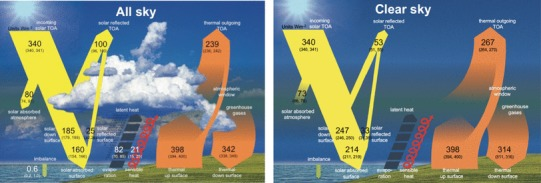
\includegraphics[scale = 7]{Chapter1_Intro/images/both_wild2019.jpg}
    \caption{The all-sky and the clear sky. Figure 14 Wild 2019. Ikke i bruk vennligst kommenter om denne er bedre enn den andre som viser differences mellom disse subplottene.}
    \label{fig:both_wild}
\end{figure}

Based on satellite and ground based measurements Wild et. al. 2019 \textbf{siter} have quantified the contribution of elements in the radiative budget. Subtracting the clear-sky from the all-sky climatology to compute the \acrfull{cre}. This is shown in equations \eqref{eq:cre_sw} and (\ref{eq:cre_lw}). Wild et. al. 2019 \textbf{siter} concludes with a reduction in shortwave radiation of $-47Wm^{-2}$ by clouds. In other words clouds reflect approximately 50\% of the incoming solar radiation. Longwave component is $28Wm^{-2}$. This give a net \acrshort{cre} of $-19Wm^{-2}$. Proving that the net effects of clouds on the radiative budget is negative.The altitude along with the composition determines the radiative properties of the cloud. \textbf{Relate this to the black body properties of clouds..? LES Artikkel fra Jonah}
\begin{figure}[h]
    \centering
    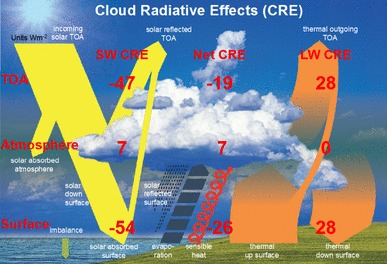
\includegraphics[scale = 7]{Chapter1_Intro/images/CRE_wild2019.jpg}
    \caption{Cloud radiative effect, CRE is the differece between the radiative components of the Clear sky radiative and the all sky. Cite this figure as fig 15 in Wild 2019}
    \label{fig:cre}
\end{figure}

\begin{equation} \label{eq:cre_sw}
    CRE_{sw} = SW\uparrow_{clear-sky} - SW\uparrow_{all-sky}
\end{equation}
\begin{equation} \label{eq:cre_lw}
    CRE_{lw} = LW\uparrow_{clear-sky} - LW\uparrow_{all-sky}
\end{equation}
\\
The physical properties causing the interaction with radiation is described below. Dense low level clouds reflect solar radiation. This is called the albedo effect. Albedo being the ratio between reflected to incoming radiation. The higher number concentrations of droplets in a cloud the higher the total surface area of droplets. The more radiation gets reflected back into space. Clouds absorb longwave radiation and re-emits it. The absorbed radiation originates from the surface and is given by Stefan-Boltzmann forth-power law, see equation (\ref{eq:stefan-boltzmann}). \textbf{En setning om at jordkloden er mye mer like en black body enn det is, vann og snø krystsller er. Selv om de også emitter som en funksjon av temp. } High clouds have low temperatures and since the re-emitted flux is a function of the cloud temperature. The greenhouse effect increases with the height of the clouds.

\begin{equation} \label{eq:stefan-boltzmann}
    F = \sigma T ^4
\end{equation}

\section{Clouds in future climates} \label{sec:intro_cloud_future_climates}
\begin{figure}[h]
    \centering
    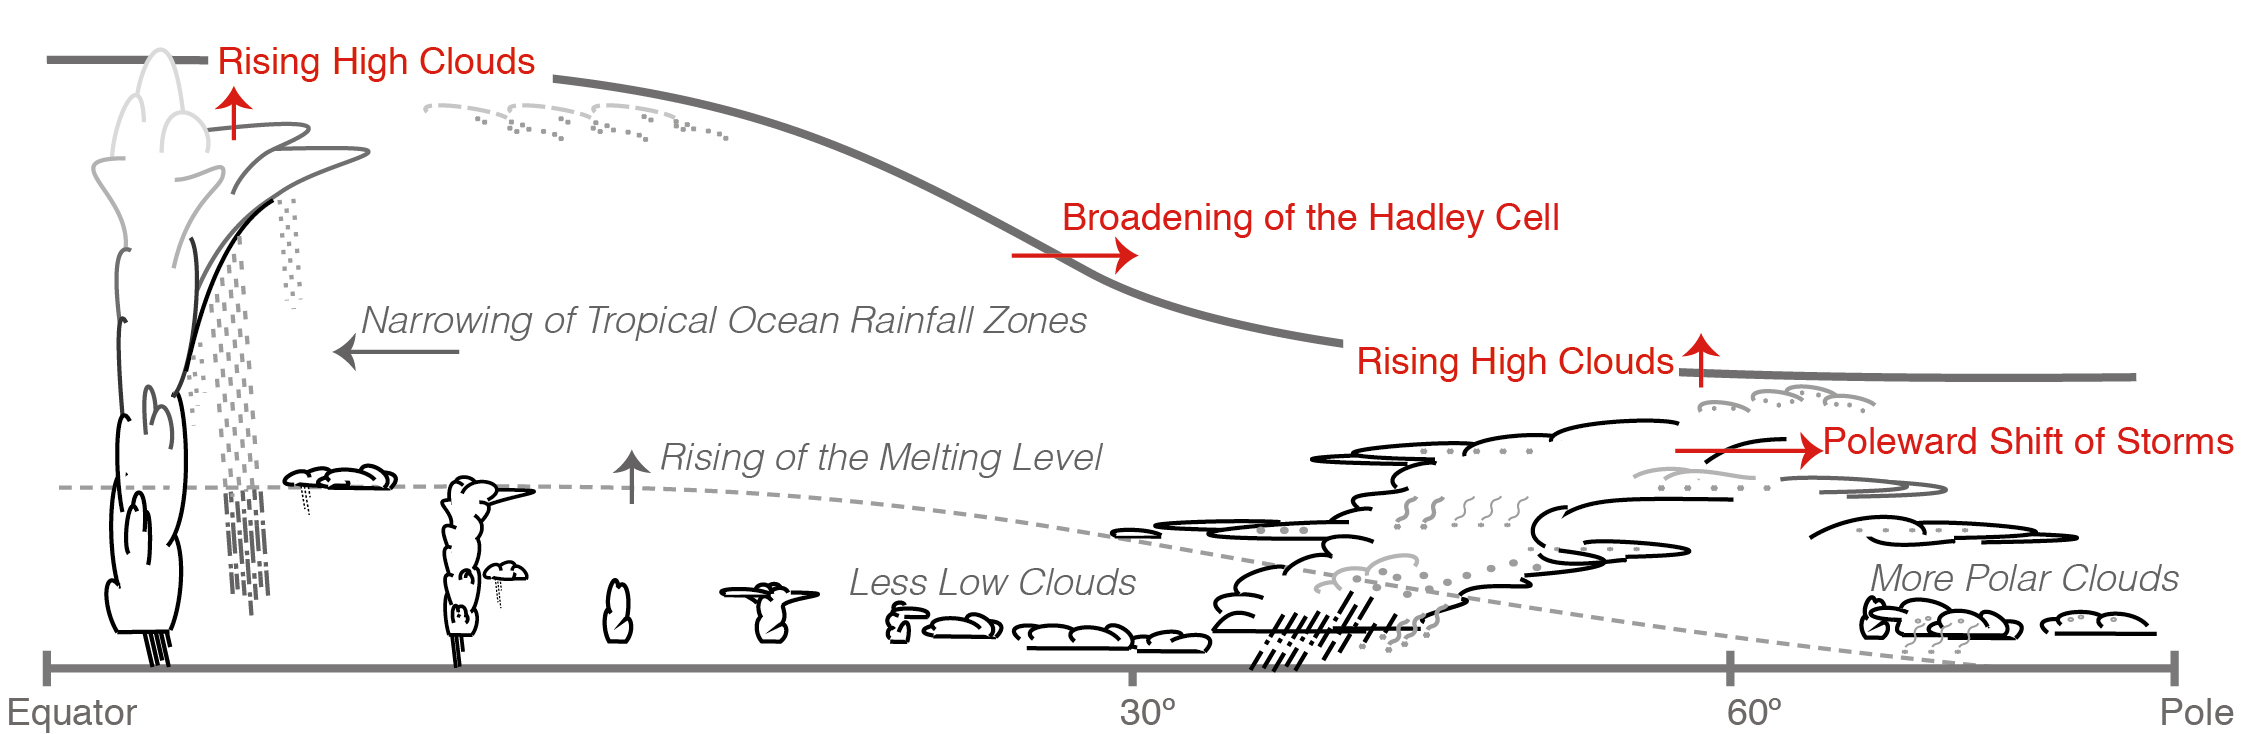
\includegraphics[scale = 0.8]{Chapter1_Intro/images/Fig7-11_ipcc.jpg}
    \caption{Cloud climatology in future climate. Developed based feedbacks in climate models, the different adjustments have different sikkerhet. Cite the fifth assessment report IPCC report.}
    \label{fig:cloud_scheme}
\end{figure}

Wild et. al. 2019  \textbf{siter} finds a imbalance of $0.6W m^{-2}$. This heat gets trapped in the earth system, forcing the surface temperature to increase in order to close the radiative budget. The imbalance in the radiative budget at \acrshort{toa} is the radiative forcing. Climate drivers include both natural and antropogentic forcings. This can be everything from natural variability in the solar energy output, vulcanic eruptions and green house gas emisions. The overall goal is to compute the climate sensitivity/equilibrium temperature as a function of forcing. For different \acrfull{rcp} scenarios one get a different temperature increase.
\\ \\ 
The global temperature will keep rising until we have reached the equilibrium climate temperature. This temperature increase induces climate changes. The \acrshort{ipcc} suggest the following shift in cloud schemes (see figure \ref{fig:cloud_scheme}). A broadening of the Hadley cell causes a poleward shift of storms. \textbf{spinn bevart lenger nord?} The albedo effect decrease at higher latitude. Moving the dense clouds further into the polar night. %Only the greenhouse effect of theses clouds persist. 
The greenhouse effect of clouds still persist without sunlight leading to a net heating in the Arctic. Rising higher clouds causing a stronger greenhouse effect of clouds.
\\ \\
Aerosols can alter the cloud micro-physics and in terms alter the radiative properties of the cloud. A polluted cloud gets extra \acrshort{ccn}, this results in more smaller droplets, as they share the available liquid. This increases the total surface area of the droplets. Which again reflect more radiation and could led to a enhanced lifetime, since it takes longer for the droplets to reach precipitation size. If it does, it might not since only one out of ten cloud precipitate. \textbf{cloud physics book} When clouds persipitate they clean the air by removing particles.
\\ \\ 
Narrowing of the Tropical ocean rainfall zones causes a drier subtropics. Rising of the meltlayer can cause the ice crystals to melt. This will results in more opaque clouds. These have a higher albedo and reflect more sunlight. \textbf{read page 591-592 again.}
\\ \\
Cloud micro-physical processes are not yet fully understood. Along with the fact that clouds are formed a smaller scale then can be resolved in your average climate models. Parametrizations are used to include the contribution from the subgridscale processes to the mesoscale proceses (weather phenomenons) in climate models and in weather predictions in general. Over the last years this has gained more attention since its acknowleged as the largest contributor to the uncertainty in climate models. I'll get back to this in chapter \ref{ch:theoretical_back}.

\section{Deep Learning} \label{sec:intro_deep_learning}
Artificial intelligence dates back to the fifties when pioneers start talking about \textit{automating task normally performed by humans}. Machine learning is a means to achieve artificial intelligence. The progress in the field follows a sigmoid curve. Slow increase at first, then really steep, before it slows down again (see figure \textbf{ref sigmoid activation func}). Over the years there have been several discoveries kick-starting the development in machine learning. The very first algorithm's include probabilistic modelling. Using the principles of statistics to analyse data. This includes Naive Bayes classifiers and logistic regression. Two algorithm's which predates computers and are still useful today. Three main bottlenecks of advances in AI is hardware, data and algorithm's. Internet continuous to provide large amounts of data from Wikipedia, Flicker (tagged images) and YouTube. Advances in computational powers, such as graphical processing units, GPU's \textit{provide a environment/platform to learn in/on}. These where originally develop for the gaming industry, but in 2007 they realised a interface called CUDA (2007) which allows for computing \textbf{find a up to date cost and flops (floating point operations per second)}. \textbf{siter Chollet bok}
\\ \\ 
For clarity, the deep in deep learning refer to the number of layers. Moving from shallow networks to deeper ones (more than 10) algorithmic advances in gradient propagation was needed. This includes activation functions, weight initialisation and optimisation schemes. I'll get back to that in section \ref{sec:intro_machine_learning}. Other advances like batch normalisation, depth wise separable convolutions attributed to the revolution of \acrshort{ai}. 
\begin{figure}[h]
    \centering
    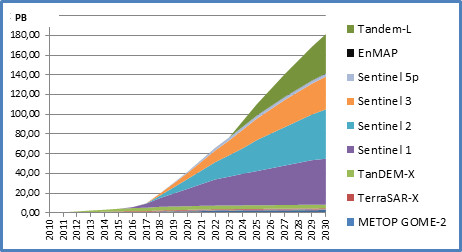
\includegraphics{Chapter1_Intro/images/Datenvolumen_D-SDA.jpg}
    \caption{Data volume. By the continuous earth system monitoring, meteorology/ climate science have progressed toward becoming a big data science. Observations are most used for verifying climate models and quantifying the current state of climate. \href{https://www.dlr.de/eoc/en/desktopdefault.aspx/tabid-12632/22039_read-51751}{https://www.dlr.de/eoc/en/desktopdefault.aspx/tabid-12632/22039{\_}read-51751}.}
    \label{fig:data_volum_sat}
\end{figure}
Earth system monitoring provides a global view of variables across meteorological systems. \textbf{Some thing about satellite era}. These large amounts of data and the flexible nature of the neural network makes is a suitable method also in geosciences. \textbf{With enough data neural networks can serve as a universal function approximate given a suitable hyper parameter tuning and input data.} The last couple of years reaserchers have been attempting to use this for wide range of problems like rainfall runoff modeling (krazerts), high-resolution weather forecasting (Rodrigues), Air quality forecasting (sun and liu), precipitaiton nowcastng (Shi et al) and \textbf{kanskje: LES} \textit{deep neural network based feature representation for weather data.} \textbf{lui et al }. \textbf{noe med forskjellig hell.} Another more comprehensive machine learning project is lead by Tapio Schneider at Caltech. Along with his team og technologist they have ambitions to create a earth system model using machine learning. With his team of from MIT and former employees of Microsoft and Google they hope to create a platform which can resolve clouds and hopefully reduce the spread in climate sensitivity. \textbf{cite science}